%%%%%%%% DATA LITERACY 2025 LATEX PROJECT TEMPLATE FILE %%%%%%%%%%%%%%%%%
%%% Based on the 2025 ICML template, available at https://icml.cc/Conferences/2025/AuthorInstructions %%%

\documentclass{article}

% Recommended, but optional, packages for figures and better typesetting:
\usepackage{microtype}
\usepackage{graphicx}
\usepackage{subfigure}
\usepackage{booktabs} % for professional tables

\usepackage{tikz}
% Corporate Design of the University of Tübingen
% Primary Colors
\definecolor{TUred}{RGB}{165,30,55}
\definecolor{TUgold}{RGB}{180,160,105}
\definecolor{TUdark}{RGB}{50,65,75}
\definecolor{TUgray}{RGB}{175,179,183}

% Secondary Colors
\definecolor{TUdarkblue}{RGB}{65,90,140}
\definecolor{TUblue}{RGB}{0,105,170}
\definecolor{TUlightblue}{RGB}{80,170,200}
\definecolor{TUlightgreen}{RGB}{130,185,160}
\definecolor{TUgreen}{RGB}{125,165,75}
\definecolor{TUdarkgreen}{RGB}{50,110,30}
\definecolor{TUocre}{RGB}{200,80,60}
\definecolor{TUviolet}{RGB}{175,110,150}
\definecolor{TUmauve}{RGB}{180,160,150}
\definecolor{TUbeige}{RGB}{215,180,105}
\definecolor{TUorange}{RGB}{210,150,0}
\definecolor{TUbrown}{RGB}{145,105,70}

% hyperref makes hyperlinks in the resulting PDF.
% If your build breaks (sometimes temporarily if a hyperlink spans a page)
% please comment out the following usepackage line and replace
% \usepackage{icml2023} with \usepackage[nohyperref]{icml2023} above.
\usepackage{hyperref}


% Attempt to make hyperref and algorithmic work together better:
\newcommand{\theHalgorithm}{\arabic{algorithm}}

% command for plotting legend colorbar of risk map figure
\newcommand{\coolwarmbox}{%
  \tikz[baseline]{
    \begin{scope}[yshift=0.1ex]
      \draw[black!70]
        (0,0) rectangle (4em,1ex);
      \shade[
        shading=axis,
        shading angle=0,
        left color=TUblue,
        middle color= TUgray,
        right color=TUgray
      ]
      (0,0) rectangle (2em,1ex);
      \shade[
        shading=axis,
        shading angle=0,
        left color=TUgray,
        middle color=TUgray,
        right color=TUred
      ]
      (1.9em,0) rectangle (4em,1ex);
    \end{scope}
  }%
}


\usepackage[accepted]{icml2025}

% For theorems and such
\usepackage{amsmath}
\usepackage{amssymb}
\usepackage{mathtools}
\usepackage{amsthm}
\usetikzlibrary{arrows.meta, positioning, calc}

% if you use cleveref..
\usepackage[capitalize,noabbrev]{cleveref}

% Todonotes is useful during development; simply uncomment the next line
%    and comment out the line below the next line to turn off comments
%\usepackage[disable,textsize=tiny]{todonotes}
\usepackage[textsize=tiny]{todonotes}


% The \icmltitle you define below is probably too long as a header.
% Therefore, a short form for the running title is supplied here:
\icmltitlerunning{Exposure-Adjusted Bicycle Crash Risk Estimation and Safer Routing in Berlin} % I think our title is not too long, hence we can use the same as for \icmltitle

\begin{document}

\twocolumn[
\icmltitle{Exposure-Adjusted Bicycle Crash Risk Estimation and Safer Routing in Berlin}

% It is OKAY to include author information, even for blind
% submissions: the style file will automatically remove it for you
% unless you've provided the [accepted] option to the icml2023
% package.

% List of affiliations: The first argument should be a (short)
% identifier you will use later to specify author affiliations
% Academic affiliations should list Department, University, City, Region, Country
% Industry affiliations should list Company, City, Region, Country

% You can specify symbols, otherwise they are numbered in order.
% Ideally, you should not use this facility. Affiliations will be numbered
% in order of appearance and this is the preferred way.
\icmlsetsymbol{equal}{*}

\begin{icmlauthorlist}
\icmlauthor{Eric Berger}{equal}
\icmlauthor{Edward Eichhorn}{equal}
\icmlauthor{Liaisan Faidrakhmanova}{equal}
\icmlauthor{Luise Grasl}{equal}
\icmlauthor{Tobias Schnarr}{equal}
\end{icmlauthorlist}

% fill in your matrikelnummer, email address, degree, for each group member
% \icmlaffiliation{first}{Matrikelnummer 7064584, MSc Machine Learning}
% \icmlaffiliation{second}{Matrikelnummer 12345678, MSc Quantitative Data Science}
% \icmlaffiliation{third}{Matrikelnummer 7320172, MSc Quantitative Data Science}
% \icmlaffiliation{fourth}{Matrikelnummer 7329274, MSc Quantitative Data Science}
% \icmlaffiliation{fith}{Matrikelnummer 7304640, MSc Quantitative Data Science}

% put your email addresses here. You can use initials to save space, 
% e.g. if you are called Max Mustermann, you can use \icmlcorrespondingauthor{MM}{max.mustermann@uni-tuebingen.de}
% DO USE YOUR UNIVERSITY EMAIL ADDRESS!
% \icmlcorrespondingauthor{EB}{eric.berger@student.uni-tuebingen.de} 
% \icmlcorrespondingauthor{EE}{first2.last2@uni-tuebingen.de}
% \icmlcorrespondingauthor{LF}{liaisan.faidrakhmanova@student.uni-tuebingen.de}
% \icmlcorrespondingauthor{LG}{luise.grasl@student.uni-tuebingen.de}
\icmlcorrespondingauthor{Tobias Schnarr}{tobias-marco.schnarr@student.uni-tuebingen.de}

% You may provide any keywords that you
% find helpful for describing your paper; these are used to populate
% the "keywords" metadata in the PDF but will not be shown in the document
\icmlkeywords{Machine Learning, ICML}

\vskip 0.3in
]

% this must go after the closing bracket ] following \twocolumn[ ...

% This command actually creates the footnote in the first column
% listing the affiliations and the copyright notice.
% The command takes one argument, which is text to display at the start of the footnote.
% The \icmlEqualContribution command is standard text for equal contribution.
% Remove it (just {}) if you do not need this facility.

%\printAffiliationsAndNotice{}  % leave blank if no need to mention equal contribution
\printAffiliationsAndNotice{\icmlEqualContribution} % otherwise use the standard text.

\begin{abstract}
We investigate bicycle crash risk on Berlin’s urban street network, addressing a key limitation of many safety analyses: raw crash counts conflate danger with demand and fail to distinguish
intrinsically risky locations from high-use roads. We combine police-reported crashes with a city-wide dataset of measured bicycle volumes to compute exposure-adjusted risk at the street-segment 
and junction levels. Aggregating risk to arbitrary routes enables comparisons that trade off safety against convenience. The result is a reproducible framework for exposure-controlled bicycle 
safety analysis and routing.\todo{rewrite/edit, when we have final results}
\end{abstract}

\section{Introduction}\label{sec:intro}
\begin{figure*}[t]
  \centering
  \includegraphics{figs/map_3_panels.pdf}
  \caption{\textbf{Safety-aware routing pipeline for the Berlin cycling network.}
  Panels (a–c) are zoomed in for readability; see \cref{sec:methods} for definitions and notation.
  (a) Police-recorded bicycle crashes in June 2021 ({\color{TUorange}points}) and street segments with measured cyclist exposure ({\color{TUgray}lines}).
  (b) Pooled segment-level relative crash risk estimated from all available data; high-risk segments in {\color{TUred}red} correspond to values above the 90th percentile of relative risk; {\color{TUdark}circles} mark junctions (degree $\ge 3$).
  (c) Shortest path ({\color{TUblue}blue}) versus a safer alternative ({\color{TUgreen}green}) selected to reduce cumulative relative route risk under a distance-detour constraint. {\color{TUocre}Filled circle} and {\color{TUocre}cross} denote origin and destination, respectively.
  }
  \label{fig:visual_app}
\end{figure*}

Cycling safety analyses often rely on raw crash counts, which conflate danger with demand: streets with high cyclist volumes tend to accumulate more incidents even when per-rider risk is low~\citep{luecken2018}. 
This obscures intrinsically risky locations and limits both targeted interventions and everyday route choice, particularly in dense urban networks such as Berlin~\citep{Uijtdewilligen01092024}.
We address this by estimating exposure-adjusted crash risk on the street network via a relative-risk formulation that separates cyclist demand from intrinsic danger and remains stable under sparse
or unevenly distributed observations (\cref{sec:methods}). Using police-recorded crashes from the German \emph{Accident Atlas} (Berlin subset)~\citep{Unfallatlas2025} together with a city-wide dataset of 
measured bicycle volumes at the street-segment level~\citep{kaiser_2025_15332147}, we estimate relative risk for individual street segments and, motivated by crash concentrations at intersections, 
derive junction-level risk by aggregating volumes from adjoining segments. These risk estimates are transformed into expected crash costs and propagated to route-level scores, enabling comparisons 
between shortest paths and safer alternatives that reduce estimated risk under comparable distance constraints (\cref{sec:results}; see \cref{fig:visual_app}). Taken together, this yields a reproducible
pipeline for estimating exposure-adjusted crash risk at street and junction levels from measured cyclist volumes, and a safety-aware routing approach under a bounded detour constraint.

\section{Data}\label{sec:data}\todo{cite source of official bike counting stations}
We combine police-recorded bicycle crashes with measured cyclist exposure for the city of Berlin. Crash data are drawn from the Berlin subset of the German \emph{Accident Atlas}~\citep{Unfallatlas2025} 
and filtered for bicycle-related incidents. Exposure is obtained from a city-wide dataset of Strava-derived bicycle volumes aggregated at the street-segment level~\citep{kaiser2025spatiotemporalgraphneuralnetwork}. 
We further perform a consistency check between Strava-derived cyclist volumes and official bicycle counting stations (see \cref{fig:segment_share}). The street network is represented as polyline segments with 
associated monthly cyclist counts. The dataset spans 2019--2023 and covers 4{,}335 street segments, 2{,}862 junctions, and 15{,}396 recorded bicycle crashes. At monthly resolution the data are sparse: 
in a typical month fewer than 5\% of segments and about 3\% of junctions record at least one crash.\todo{verify the percentages}

\begin{figure}[ht]
  \centering
  \includegraphics{figs/segment_share.pdf}
  \caption{Consistency check between official bicycle counts and Strava-derived cyclist volumes at the street-segment level (2023). Points show segment-wise shares of total annual counts; the dashed 
  line denotes equality between the two measures.}
  \label{fig:segment_share}
\end{figure}

To enable network-scale analysis, all layers are harmonized to a common street-network topology and projected coordinate reference system. Crash locations are matched to segments using nearest-segment 
assignment. Junctions are defined as nodes where at least three segments meet; crashes within a fixed radius are assigned to the nearest junction, and junction exposure is computed from incident segments.
Crashes and exposures are aggregated to monthly resolution, with segments and months of zero exposure dropped. To obtain stable risk estimates under sparse observations, monthly aggregates are pooled 
over the full study period and an Empirical Bayes approach is applied (\cref{sec:methods}). The resulting segment- and junction-level risk estimates serve as inputs to all routing analyses.

\section{Methods}\label{sec:methods}
\paragraph{Empirical Bayes relative risk and uncertainty.}
For each month $t$, let $A_{s,t}$ and $E_{s,t}$ denote the number of police-recorded bicycle crashes and measured cyclist exposure on street segment $s$. Junction crashes $A_{v,t}$ are defined as 
crashes within a fixed radius of junction $v$. Because a traversal typically contributes exposure to two incident segments, we approximate junction exposure by the half-sum of incident segment exposures,
\[
E_{v,t}=\tfrac{1}{2}\sum_{s\in\mathcal I(v)} E_{s,t},
\]
a common approach when turning movements are unavailable~\citep{hakkert2002uses,WANG2020105838}.
For notational convenience, both street segments and junctions are indexed by a generic entity index $i$, with $A_{i,t}$ and $E_{i,t}$ denoting the corresponding crash and exposure quantities.

Under a no-special-risk baseline, monthly crash incidence is assumed proportional to exposure, yielding the expected number of crashes
\[
\widehat{A}_{i,t}
= A_{\cdot t}\,\frac{E_{i,t}}{E_{\cdot t}},
\qquad
A_{\cdot t}=\sum_i A_{i,t},\ \ E_{\cdot t}=\sum_i E_{i,t},
\]
where sums are taken jointly over all segments and junctions, defining a shared baseline.
Because routing requires a stable long-run risk surface, crashes and baseline expectations are aggregated over the full study period,
\[
A_i=\sum_t A_{i,t},
\qquad
\widehat{A}_i=\sum_t \widehat{A}_{i,t},
\]
and the raw relative risk is $A_i/\widehat{A}_i$.

To stabilize estimation under sparsity, we introduce a latent relative-risk multiplier $\theta_i$ and model
\[
A_i \mid \theta_i \sim \text{Poisson}(\widehat{A}_i\,\theta_i),
\qquad
\theta_i \sim \text{Gamma}(\alpha,\alpha),
\]
where the Gamma prior (shape--rate) enforces $\mathbb{E}[\theta_i]=1$~\citep{Lord2010}. The shrinkage parameter $\alpha$ is estimated by method of moments~\citep{Morris1983}. Under the Poisson--Gamma model,
\[
\mathbb{E}[A_i] = \widehat{A}_i
\qquad\text{and}\qquad
\mathrm{Var}(A_i) = \widehat{A}_i + \frac{\widehat{A}_i^{\,2}}{\alpha}.
\]
Equating empirical and theoretical second moments across entities yields
\[
\widehat{\alpha}
=
\frac{\sum_i \widehat{A}_i^{\,2}}
{\sum_i (A_i-\widehat{A}_i)^2 - \sum_i \widehat{A}_i}.
\]
By conjugacy,
\begin{equation}
\label{eq:gamma_dist}
\theta_i \mid A_i,\widehat{A}_i
\sim \text{Gamma}(A_i+\alpha,\;\widehat{A}_i+\alpha),
\end{equation}
and the posterior mean
\[
r_i
= \mathbb{E}[\theta_i \mid A_i,\widehat{A}_i]
= \frac{A_i+\alpha}{\widehat{A}_i+\alpha}
\]
serves as the Empirical Bayes relative risk, with stronger shrinkage for entities with low expected counts~\citep{Hauer2002}. Uncertainty is quantified using $(1-\delta)$ credible intervals obtained 
from Gamma posterior quantiles.

\paragraph{Risk-weighted routing graph.}
Relative risk estimates are dimensionless and conditional on exposure. To obtain additive weights for routing, we rescale relative risk by the pooled baseline crash rate
\[
\bar{\lambda}=\frac{A_\cdot}{E_\cdot},
\qquad
A_\cdot=\sum_i A_i,\ \ E_\cdot=\sum_i E_i.
\]
The resulting routing weight is
\[
w_i=\bar{\lambda}\,r_i.
\]
We construct an undirected graph $G=(V,E)$ from the street network. Nodes correspond to segment endpoints and edges to street segments with length $\ell_e$. Each edge $e$ corresponds to a segment $s$ 
and inherits its routing weight $w_e=w_s$. Junction identifiers and weights are mapped to nodes via spatial snapping in a projected coordinate system, yielding a single risk-annotated network.

\paragraph{Safety-aware routing.}
We compare shortest-distance routes with alternatives that reduce estimated crash risk under a bounded detour. The length of a route $P$ is
\[
L(P)=\sum_{e\in P}\ell_e.
\]
To account for segment- and junction-level risk, the risk contribution of edge $e=(u,v)$ is
\[
\rho_e = w_e + \eta\,\frac{w_u+w_v}{2},
\]
where $w_u$ and $w_v$ are junction routing weights (zero for non-junction nodes) and $\eta\ge 0$ controls the contribution of junction risk. These quantities form an \emph{additive surrogate} for cumulative route risk.

For an origin--destination pair, the baseline route $P_{\text{dist}}$ minimizes $L(P)$. The safety-aware route solves
\begin{equation}
\label{eq:safe-routing}
\begin{aligned}
P_{\text{safe}}=\arg\min_{P}\ & R(P)=\sum_{e\in P}\rho_e \\
\text{s.t.}\ & L(P)\le (1+\varepsilon)\,L(P_{\text{dist}}),
\end{aligned}
\end{equation}
where $\varepsilon$ is the allowable relative detour~\citep{ehrgott2005multicriteria}. We approximate this constraint via a weighted-sum sweep: for $\lambda\in\Lambda$,
\[
P(\lambda)=\arg\min_{P}\sum_{e\in P}\bigl(\rho_e+\lambda\,\ell_e\bigr),
\]
and select among feasible candidates the route minimizing $R(P)$. Shortest paths are computed with Dijkstra’s algorithm.

\paragraph{Evaluation metrics.}
For each origin--destination pair, we report the relative length increase
\[
\Delta_L=\frac{L(P_{\text{safe}})-L(P_{\text{dist}})}{L(P_{\text{dist}})}
\]
and the relative risk reduction
\[
\Delta_R=\frac{R(P_{\text{dist}})-R(P_{\text{safe}})}{R(P_{\text{dist}})}.
\]
Pairs with $R(P_{\text{dist}})=0$ are excluded from $\Delta_R$ due to the undefined denominator. These metrics quantify the trade-off between distance and exposure-adjusted crash risk under bounded detours.

\section{Related work.}\label{sec:relatedw}
Prior work seeks to avoid conflating danger with demand by normalizing bicycle crashes by cyclist exposure~\citep{luecken2018}. City-scale studies show that exposure-normalized risk yields more
informative spatial patterns than raw crash counts and that finer temporal resolution improves inference, though persistent under-reporting in police records remains a challenge~\citep{Uijtdewilligen01092024}.
A central obstacle is obtaining reliable exposure: earlier work extrapolates city-wide volumes from sparse counters using learning-based models and multi-source features, while short-term measurement
campaigns improve predictions at unseen locations~\citep{Kaiser_Klein_Kaack_2025}. More recent efforts instead rely on street-segment datasets of measured bicycle volumes, enabling safety analyses 
without explicit exposure modeling~\citep{kaiser2025spatiotemporalgraphneuralnetwork}. At the network level, risk is typically defined as crashes per unit exposure on links, with attention to spatial
snapping, assignment of incidents to intersections, and integration of safety metrics into routing under convenience constraints~\citep{isprs-archives-XLIII-B4-2022-427-2022}. Intersection safety is 
repeatedly emphasized, with strong crash concentrations at junctions and the need to control for exposure when comparing locations or infrastructure types~\citep{futuretransp1030037}.

In contrast, we combine measured segment-level exposure with joint segment–junction risk estimation and propagate these risks into safety-aware routing.\todo{this sentence can be dropped if space is an issue}

\section{Results}\label{sec:results}
One of the major outcomes of this work ist the estimation of the risk to have get injured in a bike accidents while driving on a streetsegment.
This distribution of those calculated risks is displayed in \cref{fig:risk_segments}.

\begin{figure}[ht]
  \centering
  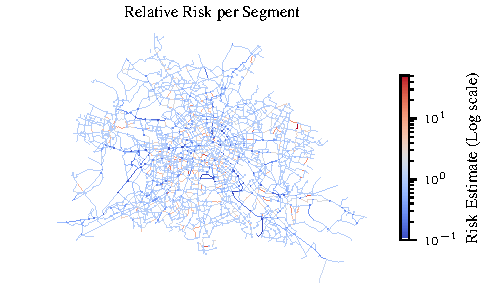
\includegraphics{figs/risk_segments.pdf}
  \caption{Risk levels across segments and junctions in the Berlin area. Colors (\coolwarmbox) represent the log-scaled risk, ranging from blue (low risk) to red (high risk).}
  \label{fig:risk_segments}
\end{figure}

To evaluate the routing algorithm, we sample $n=1000$ origin--destination pairs uniformly at random and compare shortest-distance routes with safety-aware alternatives~\citep{NateraOrozco2020}.

\begin{table}[ht]
\centering
\caption{Distance--risk trade-off under bounded detours for different junction-risk weights $\eta$.
Values are aggregated over all origin--destination pairs.
Medians are reported with interquartile ranges in parentheses.
$P(\Delta_R > 0)$ is reported in percent.}
\label{tab:routing_tradeoff}
\begin{tabular}{@{}c c c c c@{}}
\toprule
$\eta$ & $\varepsilon$ & Med.\ $\Delta_L$ & Med.\ $\Delta_R$ & $P(\Delta_R>0)$ \\
\midrule
0.0 & 0.05 & 0.009 (0.026) & 0.246 (0.451) & 76.1 \\
    & 0.10 & 0.025 (0.042) & 0.377 (0.388) & 86.0 \\
    & 0.20 & 0.038 (0.072) & 0.425 (0.353) & 90.6 \\
\addlinespace
0.5 & 0.05 & 0.008 (0.026) & 0.208 (0.401) & 75.3 \\
    & 0.10 & 0.026 (0.046) & 0.331 (0.370) & 86.4 \\
    & 0.20 & 0.047 (0.089) & 0.404 (0.323) & 92.0 \\
\addlinespace
1.0 & 0.05 & 0.008 (0.026) & 0.185 (0.363) & 75.9 \\
    & 0.10 & 0.028 (0.047) & 0.305 (0.345) & 86.3 \\
    & 0.20 & 0.050 (0.086) & 0.378 (0.318) & 91.8 \\
\bottomrule
\end{tabular}
\end{table}

\cref{tab:routing_tradeoff} summarizes the trade-off between route length and exposure-adjusted crash risk under bounded detours. Safety-aware routing identifies feasible alternatives for all 
origin--destination pairs across detour budgets and junction-risk weights.

Allowing a 10\% detour reduces exposure-adjusted crash risk by 31--38\% in median, with over 86\% of routes achieving a risk reduction for all values of the junction-risk weight. Larger detours 
further increase these gains, reaching median reductions of 38--43\% at $\varepsilon=0.20$, while even small detours ($\varepsilon=0.05$) yield measurable reductions of 18--25\%. Across all detour
budgets, increasing $\eta$ is associated with lower median risk reductions.


\section{Discussion and Conclusion}\label{sec:conclusion}
% Use this section to briefly summarize the entire text. Highlight limitations and problems, but also make clear statements where they are possible and supported by the analysis. 
Our results indicate that substantial reductions in exposure-adjusted crash risk can be achieved with relatively small increases in route length. While higher junction-risk weights reduce the magnitude
of the estimated risk reduction, the distance--risk trade-off persists across all configurations, with absolute gains depending on the chosen weighting.

Overall, allowing a 10\% increase in route length yields median exposure-adjusted risk reductions of 31--38\% for the majority of routes, demonstrating that safety-aware routing can effectively trade 
modest detours for meaningful safety improvements.


We provide implementation details, hyperparameters, and supplementary material, available at \url{https://github.com/ytobiaz/data_literacy}.

\clearpage

\section*{Contribution Statement}
Explain here, in one sentence per person, what each group member contributed. For example, you could write: Max Mustermann collected and prepared data. Gabi Musterfrau and John Doe performed the data analysis. Jane Doe produced visualizations. All authors will jointly wrote the text of the report. Note that you, as a group, a collectively responsible for the report. Your contributions should be roughly equal in amount and difficulty.

% \section*{Notes} 
% Your entire report has a \textbf{hard page limit of 4 pages} excluding references and the contribution statement. (I.e. any pages beyond page 4 must only contain the contribution statement and references). Appendices are \emph{not} possible. But you can put additional material, like interactive visualizations or videos, on a githunb repo (use \href{https://github.com/pnkraemer/tueplots}{links} in your pdf to refer to them). Each report has to contain \textbf{at least three plots or visualizations}, and \textbf{cite at least two references}. More details about how to prepare the report, inclucing how to produce plots, cite correctly, and how to ideally structure your github repo, will be discussed in the lecture, where a rubric for the evaluation will also be provided.


\bibliography{bibliography}
\bibliographystyle{icml2025}

\end{document}

% This document was modified from the files available at https://icml.cc/Conferences/2025/AuthorInstructions
% the full copyright notice is available within the file icml2025.sty